%ju 13-Aug-22 06-Klimaanlage.tex
\section{Aktive und Passive
Sicherheit}\label{aktive-und-passive-sicherheit}

\textbf{Aktive Sicherheit} Maßnahmen zur Vermeidung von Unfällen

\begin{itemize}
\item
  \emph{Beispiele:} ABS, ESP, Klima, Scheibenwischer, ACC (adaptive
  Geschwindigkeitsregelung)
\end{itemize}

\textbf{Passive Sicherheit} Maßnahmen zur Minderung von Unfallfolgen

\begin{itemize}
\item
  \emph{Beispiele:} Airbag (Fahrer-, Beifahrer-, Kopf- und
  Seitenairbags), Gurtstraffer, Batterietrennschalter (Kurzschluss,
  Brandgefahr), Motorhaubenaufsteller
\end{itemize}

\textbf{Airbag löst nach} ca. $15 - 50~ms$ aus (Zündung --
Entfaltung), Crashsensoren: max. $30^\circ$ Aufprallwinkel zur
Längsachse

\textbf{Gurtstraffer zieht Gurt nach} ca. $20 - 25~ms$ bis zu
$15~cm$ ein.

\section{Aufbau und Funktionsweise einer
Klimaanlage}\label{aufbau-und-funktionsweise-einer-klimaanlage}

\textbf{Luftgütesensor:} misst Schadstoffe in der Außenluft (Frischluft
vs.~Innenraumluft)

\textbf{Wärme} vs.~\textbf{negative Wärme} (Kälte)

\textbf{Enthalpie} Element, das eine bestimmte Wärmeenergie hat

\textbf{Komponenten}

\begin{enumerate}
\item
  \textbf{Magnetkupplung} Verbindung zwischen Riemenscheibe und
  Antriebswelle

  \begin{itemize}
  \item
    Spaltmaß: $0,4 - 0,6~mm$
  \end{itemize}
\item
  \textbf{Kompressor} Kältemittel verdichten

  \begin{itemize}
  \item
    Taumelscheibenverdichter (Förderleistung variieren)
  \item
    Flügelzellenverdichter
  \item
    Spiralverdichter (Hybrid- und Elektrofahrzeuge)
  \item
    Kompressor mit variablem Hub und externer Regelung (PWM-Signal)
  \end{itemize}
\item
  \textbf{Trockner} Kältemittel trocknen, filtern, beruhigen, Sammler
\item
  \textbf{Expansionsventil} regelt Kältemittelzufluss zum Verdampfer, um
  zu verhindern, dass der Kompressor flüssiges Kältemittel ansaugt
  (Flüssigkeitsschlag)
\item
  \textbf{Druckschalter und Überdruckventil} Schutz der Klimaanlage

  \begin{itemize}
  \item
    Kühlerlüfter / Kondensatorgebläse

    \begin{itemize}
    \item
      EIN: $\sim 16~\text{bar}$, AUS: $\sim 10~\text{bar}$
    \end{itemize}
  \item
    Magnetkupplung

    \begin{itemize}
    \item
      Druckschalter: Druck zu niedrig $\sim 2~\text{bar}$, Druck zu
      hoch $\sim 28~\text{bar}$
    \end{itemize}
  \item
    Verdampfersonde / Vereisungssensor

    \begin{itemize}
    \item
      Vereisungsschutz EIN $> +4^\circ \text{C}$, AUS
      $< 0^\circ \text{C}$
    \end{itemize}
  \end{itemize}
\end{enumerate}

\textbf{Funktion}

Kältemittel nimmt Energie auf und gib sie wieder ab bei Änderung seines
Aggregatzustandes.

Bei geringem Druck und niedriger Temperatur verdampft Kältemittel. Der
Siedepunkt kann durch Druckänderung verschoben werden. Erhöht man den
Druck, dann steigt die Verdampfungstemperatur.

Beispiel: R134a

\begin{itemize}
\item
  Atmosphärische Druck: ca. $1~\text{bar} \to$ Siedepunkt: ca.
  $-26^\circ \text{C}$
\item
  Überdruck: ca. $15~\text{bar} \to$ Siedepunkt: ca.
  $55^\circ \text{C}$
\end{itemize}

\textbf{Verdampfer} verdampfen, Energie aufnehmen, \emph{Wärme\_zu}, aus
der Umgebung wird Wärme entzogen. Notwendig, wenn man eine Flüssigkeit
verdampfen möchte. (flüssig $\to$ gasförmig)

vs.

\textbf{Kondensator} kondensieren, Energie abgeben, \emph{Wärme\_ab} an
die Umgebung (gasförmig $\to$ flüssig)

\textbf{Wärmepumpe} Heizen (PTC) und Kühlen

\section{Kältemittelkreislauf}\label{kaeltemittelkreislauf}

\begin{figure}[!ht]% hier: !ht
\centering
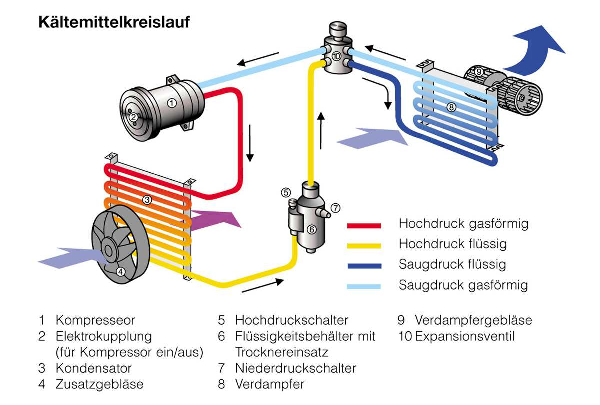
\includegraphics[width=0.5\textwidth]{images/Skizze/Klimakreislauf-1.pdf}
\caption{Klimakreislauf}
%\label{fig:}%% anpassen
\end{figure}

\begin{enumerate}
\item
  \textbf{Kompressor} (Gasverdichter, Komprimieren, Druck steigt,
  gasförmig) der kalte Dampf (gasförmig) wird abgesaugt und verdichtet.
  Dadurch steigt Druck und Temperatur des Gases.

  \begin{itemize}
  \item
    Umlauf des Kältemittels
  \item
    Fördermenge beeinflusst Kälteleistung
  \end{itemize}
\item
  \textbf{Kondensator} (Verflüssiger, Kondensieren) das unter hohen
  Druck stehende heiße Gas wird in den Kondensator gepresst. Durch den
  Fahrtwind / Lüfter wird das heiße Gas abgekühlt und verflüssigt. Je
  besser gekühlt wird, desto geringer der Druck.

  \begin{itemize}
  \item
    Aggregatzustandswechsel: gasförmig $\to$ flüssig (Druck ist
    konstant)
  \item
    \textbf{Trockner} flüssiges Kältemittel wird entfeuchtet und
    gefiltert.
  \end{itemize}
\item
  \textbf{Expansionsventil} (Dosiereinheit, Druckminderer, Drossel,
  Expandieren, flüssig) Kältemittel expandiert (Druck sinkt) und regelt
  die Menge des Kältemittels zum Verdampfer.
\item
  \textbf{Verdampfer} (Verdampfen) warme Luft bringt das entspannte
  flüssige Kältemittel bei geringer Temperatur zum Verdampfen. Dabei
  entzieht das Kältemittel der Luft Wärme und kühlt sie ab.

  \begin{itemize}
  \item
    Aggregatzustandswechsel: flüssig $\to$ gasförmig (Druck ist
    konstant)
  \end{itemize}
\end{enumerate}

\section{Klimaservice}\label{klimaservice}

\textbf{Ruhedruck} (Motor aus)

\begin{itemize}
\item
  Kältemitteldruck abhängig von Umgebungstemperatur (Vgl. Dampftafel /
  Richtwerte \textcite{schmidt:2015:klima} S. 120)
\end{itemize}

\textbf{Betriebsdruck} (Motor an im LL, Klima ON, max. Gebläse, Keine
Umluft, Heizung OFF, Temp. LOW, $5 - 10~\text{Min.}$ laufen lassen)

\begin{itemize}
\item
  \textbf{Sollwerte} Quelle: Andreas Lamm \footnote{\url{https://klimacheck.com/}}
\item
  ND $1 - 3~\text{bar}$
\item
  HD $7 - 20~\text{bar}$
\item
  Kühlung

  \begin{itemize}
  \item
    Außentemperatur $20^\circ \text{C} \to 2 - 8^\circ \text{C}$
    \textbf{Ausströmtemperatur}
  \item
    Außentemperatur $30^\circ \text{C} \to \, <15^\circ \text{C}$
    Ausströmtemperatur
  \end{itemize}
\end{itemize}

\textbf{Klimadiagnose}

\begin{enumerate}
\item
  Betriebsdruck (Vgl. Sollwerte)

  \begin{itemize}
  \item
    \textbf{Läuft Kondensatorlüfter?}

    \begin{itemize}
    \item
      Wenn Defroster EIN, dann muss Lüfter laufen!
    \end{itemize}
  \end{itemize}
\item
  Ausströmtemperatur (Vgl. Sollwerte)
\item
  Zustand Kältemittel (Schauglas)
\end{enumerate}

\emph{Vgl. Diagnosetabelle}

\begin{table}[!ht]% hier: !ht 
\centering 
	\caption{}% \label{tab:}%% anpassen 
\begin{tabular}{@{}lll@{}}
\hline
\textbf{Hochdruck} & \textbf{Niederdruck} & \textbf{Ursache} \\
\hline
normal, zu hoch & zu niedrig & Expansionsventil, Filter, Kondensator \\
normal, zu niedrig & zu hoch & zu viel Kältemittel, Kompressor \\
normal, zu niedrig & zu niedrig & zu wenig Kältemittel,
Magnetkupplung \\
zu niedrig & zu hoch & zu viel Kältemittel, Kondensator,
Kondensatorlüfter \\
\hline
\end{tabular} 
\end{table}

Anhand der Leitungstemperaturen auf mögliche defekte im
Kältemittelkreislauf schließen (\textcite{schmidt:2015:klima} S. 115).

Übersicht über fehlerhafte Füllmengen und Komponenten die sich an den
Druckmanometern widerspiegeln können (\textcite{schmidt:2015:klima} S. 116
-- 117).

\textbf{Magnetkupplung am Kompressor prüfen}

\begin{enumerate}
\item
  Spannungsversorgung prüfen (Verkabelung, Sicherung, Relais)

  \begin{enumerate}
  \def\labelenumii{\arabic{enumii}.}
  \item
    Magnetkupplung (Spannung am Verbraucher) Soll: $12~V$
  \item
    Masseanschluss (gegen Masse) Soll: $0~V$
  \item
    Relais (gegen Masse) Soll: $12~V$
  \item
    Druckschalter (gegen Masse) Soll: $12~V$
  \end{enumerate}
\item
  Temperatur- und Druckschalter, Steuergerät, Luftspalt
\end{enumerate}

\textbf{Kondensatorlüfter prüfen}

\begin{itemize}
\item
  Sicherung, Relais, Verkabelung, Motor, Schwergängigkeit
\end{itemize}

\textbf{Klima-Service-Gerät}

\begin{itemize}
\item
  Vakuumzeit
  $\boxed{60~Min/kg \cdot \text{Kältemittelmenge [kg]}} \quad (1~h~\hat =~ 1~kg)$
\item
  Füllung
\item
  Kompressor-Öl
\end{itemize}

Phasen

\begin{enumerate}
\item
  \textbf{Absaugen} (von Kältemittel und Kompressoröl)
\item
  \textbf{Evakuieren} (Vakuum, Wasser entfernen, Dichtigkeit prüfen)
\item
  \textbf{Aufbereiten} (Kältemittel von Wasser und Öl trennen und
  wiegen)
\item
  \textbf{Auffüllen} (von Kältemittel und Kompressoröl)
\end{enumerate}

\textbf{Verlust an Kältemittel}
$[\%] \, \boxed{= \frac{\text{abgesaugte Menge}}{\text{Füllmenge}} \cdot 100} \quad \text{Beispiel: } \frac{180~g}{640~g} \cdot 100 = 28~\%$

Jährlich ca. $10~\%$ Verlust normal.
